\documentclass[a4paper,10pt,twoside]{report}
\usepackage{relsize}
\usepackage{graphicx}
\usepackage{longtable}
\usepackage{multirow}
%\usepackage[colorlinks,citecolor=red,urlcolor=red]{hyperref}
\usepackage{listings} %% ENRIQUE: para sacar listados en bonito.
\usepackage[plainpages=false,pdfpagelabels,bookmarksopen,bookmarksnumbered,linkcolor=blue,colorlinks=true,citecolor=blue,urlcolor=blue]{hyperref}


\lstloadlanguages{C,Ada}
\lstset{language=C}
\lstset{numbers=left}


%% The default sizes of LaTeX is too small. It is better to put more
%% stuff on each page!.
\setlength{\textwidth}{6.78in}
\setlength{\textheight}{8.9in}
\setlength{\hoffset}{-0.25in} % 0,75in margin
\setlength{\voffset}{-0.50in} % 0,50in margin
\setlength{\oddsidemargin}{0in}
\setlength{\evensidemargin}{\oddsidemargin}
\setlength{\headheight}{0.20in}
\setlength{\footskip}{0.60in}
\setlength{\headsep}{0.31in}


%\def\PartiKle{%
%  P\kern-.30em%
%  {\relsize{-0.5}\raisebox{-.3ex}[0ex][0ex]{a}\raisebox{0.0ex}{r}\raisebox{.2ex}{t}\raisebox{.4ex}{i}}K\kern-.10em%
%  {\relsize{-0.5}l\raisebox{-.5ex}[0ex][0ex]{e}} %
%}
%\newcommand\partikle{%
%  P\kern-.30em%
%  {\relsize{-0.5}\raisebox{-.3ex}[0ex][0ex]{a}}%
%  {\relsize{-2.7}RT}%
%  {\relsize{-0.0}{i}}K%
%  {\relsize{-0.5}l\raisebox{-.5ex}[0ex][0ex]{e}} %
%}
\newcommand{\partikle}[0]{PaRTiKle}
\newcommand{\xtratum}[0]{XtratuM}

% Title Page
\title{\partikle{} users manual}
\author{M. Masmano, I. Ripoll, A. Crespo}

\begin{document} 
\maketitle

\begin{abstract}
To be written.
\end{abstract}
\chapter{Introduction}
\section{\partikle{} Overview}
\partikle{} is a new open source real-time kernel for embedded systems,
distributed under the terms of the GNU Public License. It is important
to note that applications that use \partikle{} system calls are not
considered as \textit{derived work}; therefore, \partikle{} applications
do not need to be GPL or even GPL compatible\footnote{Although we
  recomend to use GPL.}.  It is also royalty and buyout free. In
short, \partikle{} license schema is the same that the one used in the
Linux kernel. If you can write Linux applications then you can write
\partikle{} applications.

It is a full-featured, flexible, configurable, real time embedded
kernel. The kernel provides thread scheduling, synchronization, timer,
and communication primitives. It handles hardware resources such as
interrupts, exceptions, memory, timers, etc.
 
% \partikle{} can be build to run on three diferent execution environments:
% \begin{itemize}
% \item As a stand-alone system on a bare machine (very low footprint).
% \item As a regular Linux process (for testing purposes).
% \item As a \xtratum{} domain (which allows to run Linux and \partikle{} at
%   the same time on the same computer).
% \end{itemize}

\partikle{} was designed to be POSIX compatible. The native API is ``C''
POSIX threads. But also, provides support for C++, Ada and Java
(tasking, synchronisation, protected objects, exception handling,
etc.).  Besides POSIX compatibility, \partikle{} also provides the
RTLinux/GPL non-portable POSIX extensions; therefore, it should be
possible to compile RTLinux/GPL applications on \partikle{} to get all
the benefits.


\partikle{} has been initially developed by the Real-Time Systems
Group\footnote{\url{http://www.gii.upv.es}} of the Universidad
Politecnica de Valencia\footnote{\url{http://www.upv.es}}, Spain.

% \partikle{} is provided as an open source runtime system supported by the
% GNU open source development tools. Developers have full and unfettered
% access to all aspects of the runtime system. No parts of it are
% proprietary or hidden, and you are at liberty to examine, add to, and
% modify the code as you deem necessary. These rights are granted to you
% and protected by the GNU Public License (GPL).

\partikle{} has been designed to support applications with real-time
requirements, providing features such as full preemptability, minimal
interrupt latencies, and all the necessary synchronization primitives,
scheduling policies, and interrupt handling mechanisms needed for
these type of applications.

At this moment, \partikle{} is available for i386 processors and the
runtime can be configurated for three different execution
environments:
\begin{itemize}
\item As a stand-alone system on a bare machine: The generated code
  (runtime plus application) can be executed directly on i386 boards.
  See section~\ref{config} for GRUB configuration.
\item As a Linux process: This environment is intented for testing
  purposes. The generated code is be executed as a regular Linux
  process.
\item As a \xtratum{} domain: \xtratum{} is an hypervisor that provides
  hardware virtualisation and allows to execute several kernels (or
  run-times) concurrently. \partikle{} can be built to be \xtratum{} aware
  and then executed in a \xtratum{} domain.
\end{itemize}

The last execution environment provides an execution framework which
is very close to that provided by RTLinux/GPL, RTAI and Xenomai. In
this case, applications written for RTLinux/GPL should run on
\xtratum{}+\partikle{} with minor modifications.

\chapter{PaRTiKle installation}
\section{System requirements}


The development environment requires Intel architecture PC running
Linux. Disk space requirements are minimal (less than 1Gb).

Compiler and tools that are known to be needed:
\begin{itemize}
\item GCC 3.4 or 4.0 for kernel and ``C'' applications.
\item GNAT 2005 compiler for Ada applications.
\item C++  3.4 (with 4.x is known not to work\footnote{The DWARF
    support has been changed and is not backward compatible.})
\item Java 3.4 (with 4.x is known not to work for the same reasons
  that for C++).
\item Make
\item ncurses (5.0 or above).
\item bash
\end{itemize}



Since  it  is  not possible  to  test  the  compatibility of  all  the
developing tools, bellow is a list of the tools/versions used to build
\partikle{}. We  use have used kubuntu  6.06.1. Note that  since the Ada
compiler is not  included in most distributions for  legal reasons, it
has            to             be            downloaded            from
AdaCore\footnote{\url{http://www.adacore.com/home/academia/gap}}.




\begin{table}[htb]\centering
\begin{tabular}{l|l}\hline
Gnu C       &           3.4.6 \\ 
Gnu make    &           3.81beta4\\
binutils    &           2.16.91\\
util-linux   &          2.12r\\
module-init-tools &     3.2.2\\
Linux C Library   &     2.3.6\\
Dynamic linker (ldd) &  2.3.6\\
Procps            &     3.2.6\\
Net-tools         &     1.60\\
Console-tools     &     0.2.3\\
ncurses-lib    & 5.0\\ \hline
\end{tabular}
\caption{Summary of tools that are known to compile PaRTiKle.}
\end{table}

Due to the rapid and continuous development of the GNU ``C'' compiler
it is possible (and common) to have installed and operative several
compiler versions. By default, the path of the compiler used by
PaRTiKle is \texttt{/usr/bin/gcc}, which is a link to the actual
executable. Many distributions let the responsibility of creating this
link to the user. You have to create the link with:
\begin{verbatim}
# ln -s /usr/bin/gcc-3.4 /usr/bin/gcc
\end{verbatim}

Also if you have a Debian or Ubuntu distribution, then you can update
the link with:
\begin{verbatim}
# update-alternatives --install /usr/bin/gcc gcc /usr/bin/gcc-3.4 1
\end{verbatim}



\partikle{} can be downloaded from \url{http://rtportal.upv.es/partikle}.
%%%%%%%%%%%%%%%%%%%%%%%%%%%%%%%%%%%%%%%%%%%%%%%%%%%%%%%%%%%%
\subsection{PaRTiKle configuration}
%%%%%%%%%%%%%%%%%%%%%%%%%%%%%%%%%%%%%%%%%%%%%%%%%%%%%%%%%%%%

In the \partikle{} directory, execute the configuration menu.
\begin{verbatim}
$ make menuconfig
\end{verbatim}
In this menu you can configure: 


The first option, \texttt{Target}, allows to select your target
execution environment.

Enabling ``Verbose Compiling'' will display complete information
during the compilation process. All that output information is usually
not needed except for developers. It is advisable to disable this
option.

If you plan to debug your application with a run time code debugger
then you have to enable ``Debugging support'' option to add debugging
symbols to the final executable.

If you select a language support, paths for compiler and linker has
to be provided.
\begin{figure}[htbp]\centering
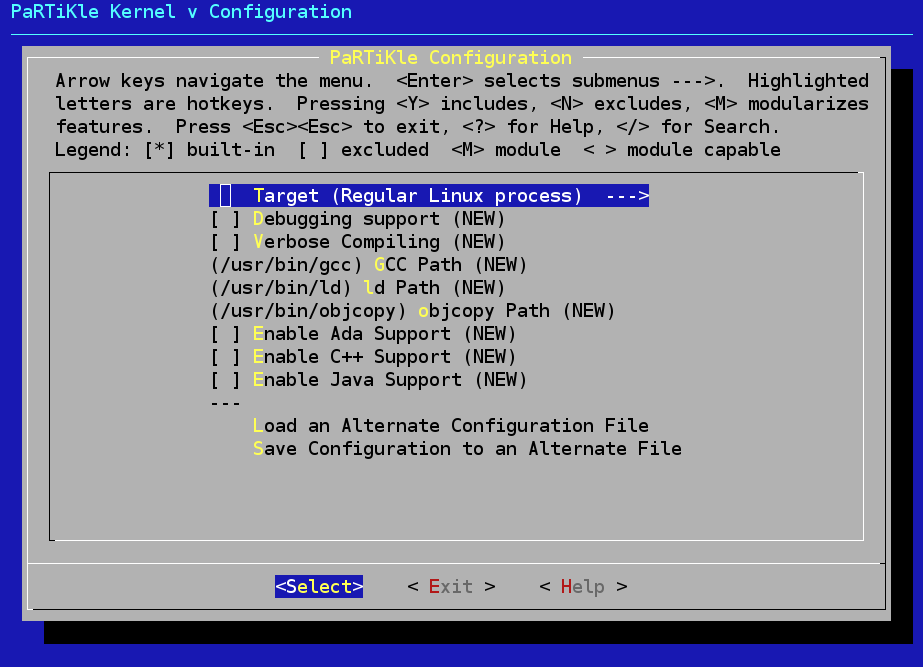
\includegraphics[width=0.49\textwidth]{img/config1}
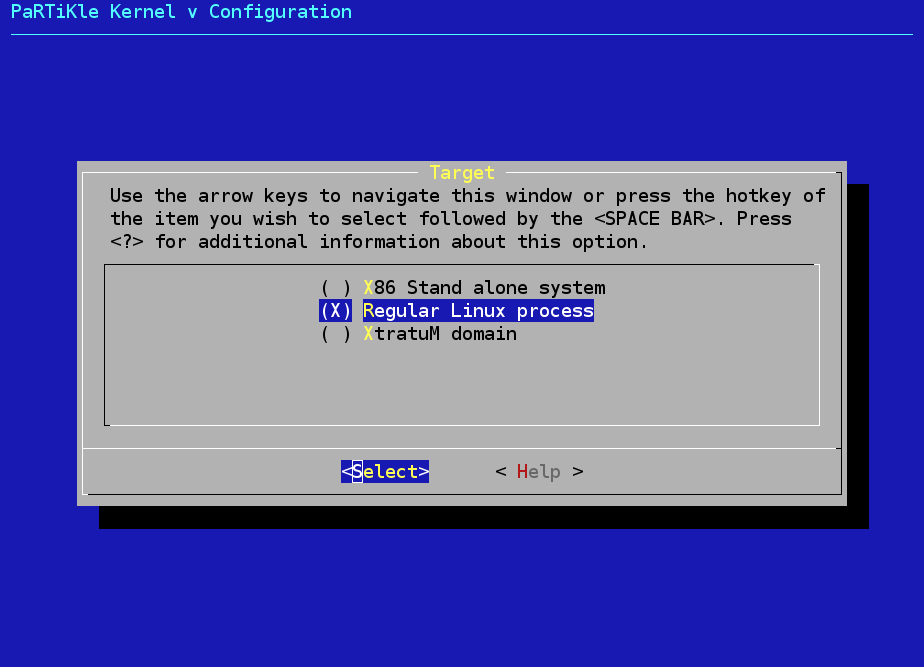
\includegraphics[width=0.49\textwidth]{img/config2}
\caption{Configuration screen-shoots.}
\label{img:config1}
\end{figure}

%%%%%%%%%%%%%%%%%%%%%%%%%%%%%%%%%%%%%%%%%%%%%%%%%%%%%%%%%%%%
\subsection{PaRTiKle building}
%%%%%%%%%%%%%%%%%%%%%%%%%%%%%%%%%%%%%%%%%%%%%%%%%%%%%%%%%%%%



\partikle{} has to be compiled to generate the code for the selected configuration.
\begin{verbatim} 
$ make

>> Target architecture: [xm_i386]:
..
>> Building the PaRTiKle kernel:
..........................
>> Building languages support:
 > DWARF2 support: ...
 > Ada support: ..

>> PaRTiKle done.
\end{verbatim}

The result of the compilation process is a file called
\texttt{core/partikle\_core.o} that is an object file which contains
the kernel selected; and a set of libraries
(\texttt{user/ulibc/libc/ulibc.a},
\texttt{user/lang\_support/gcc/libgcc\_eh.a},
\texttt{user/lang\_support/libsupc++.a}, etc.) which depends on the
selected languages.

Now you can test \partikle{} by running some examples. To compile and
build the example, follow these steps:
\begin{enumerate}
\item Go to \texttt{user/examples/c\_examples} folder.
\item Run the the \texttt{make} command.
\item The build process creates a file with named
  \textit{[example]}\texttt{.prtk} for each example, which
  contains the \partikle{} kernel and the application example.
\end{enumerate}

\label{config}
The way to launch the application depends on the target execution
environment:
\begin{description}
\item[Stand-alone] The \partikle{} system is, in this case, a multi-boot
  compliant ELF file. Copy the file to the \texttt{/boot} directory of
  the target machine; and add the following lines to the grub
  configuration file \texttt{/boot/grub/menu.lst} (assuming that the
  folder \texttt{/boot} is located in the first partition of the first
  ATA disk):
\begin{verbatim}
title           PaRTiKle
root            (hd0,0)
kernel          /boot/example.prk
boot
\end{verbatim} 
   
  Then reboot the target computer and select the PaRTiKle boot target.
  
\item[\xtratum{} domain] The target Linux system has to be modified and
  recompiled to support \xtratum{} (the reader is referred to the \xtratum{}
  installation instructions). The \xtratum{} module (\texttt{xm.ko}) has
  to be loaded before \partikle{} system can be launched. Use the
  \texttt{loader.xm} utility to load the \partikle{} system (supposing
  that \texttt{XM} variable points to the \xtratum{} directory):
\begin{verbatim}
# insmod $XM/xm.ko
# $XM/user_tools/xmloader/loader.xm example.prtk
\end{verbatim}
\item[Linux process] In this case, the \partikle{} application is a
  normal Linux executable:
\begin{verbatim}
# ./example.prtk
\end{verbatim}
\end{description}


\section{Application building}

PaRTiKle provides a script, named \texttt{ldkernel}, to ease the
building process of PaRTiKle's applications. This script syntax is:

\begin{verbatim}
$ ldkernel -f <output> <file1.o> [<file2.o> ...]
\end{verbatim}
 
where \verb#<output># is the name of the target executable, and
\verb#<file1.o>#, \verb#<file2.o>#, etc., are the object files
obtained when the application is compiled using GCC with the option
\texttt{-c}.

The steps perfomed by this script are:

\begin{enumerate}
\item It links the application jointly with the user ``C'' library and
  the suitable run-time (the run-time is selected depending on the
  language used to implement the application).
\item It turns every application's symbol into a local symbol, except
  \textit{start\_user\_app}.
\item Eventually, the script links the resulting object file together
  with the kernel object file to create the executive.
\end{enumerate}

For example, to compile the example~\ref{partikle:example}
(implemented in the file \texttt{example.c}), we should compile this
file using GCC with the next flags:
\begin{table}[h]\centering
\begin{tabular}{ll}
\multicolumn{1}{c}{FLAG}  & \multicolumn{1}{c}{Comment} \\ \hline
  \texttt{-Wall}         & enable all warning messages.\\
  \texttt{-O2}           & optimize for speed (advisable).\\
  \texttt{-c}            & do not link (the \texttt{ldkernel} script will do it).\\
  \texttt{-fno-builtin}  & do not use compiler builtin functions (cross
  compiling) \\
  \texttt{-nostdlib}     & use only the \partikle{} specific libraries.\\
  \texttt{-nostdinc}     & use only the \partikle{} include files.\\
  \texttt{-Dxm\_i386}    & declare the execution environment used.\\
  \texttt{-I\textit{<PaRTiKle>}/user/ulibc/include} & use PaRTiKle includes.\\
  \texttt{-fomit-frame-pointer} &  the frame pointer (\texttt{EBP}) is
  not needed. \\ \hline
\end{tabular}
\end{table}
The line that has to be issued to comple \texttt{example.c} is:

\begin{verbatim}
# gcc -Wall -O2 -c -fno-builtin -nostdlib -nostdinc -Dxm_i386 \
      -I<PaRTiKle>/user/ulibc/include \
      -fomit-frame-pointer -o example.o example.c 
\end{verbatim}

The the application contains more than one source file, then each file
has to be compiled separately and then linked together with the
\texttt{ldkernel} script.

After that, we invoke the \texttt{ldkernel} script as follows:

\begin{verbatim}
$ ldkernel -o example.prtk example.o
\end{verbatim}

The result is a file named \texttt{example.prk}, ready to be executed
in the selected execution environment. Figure~\ref{img:building}
sumarises the whole process of building a PaRTiKle system.

\begin{figure}[tbhp]\centering
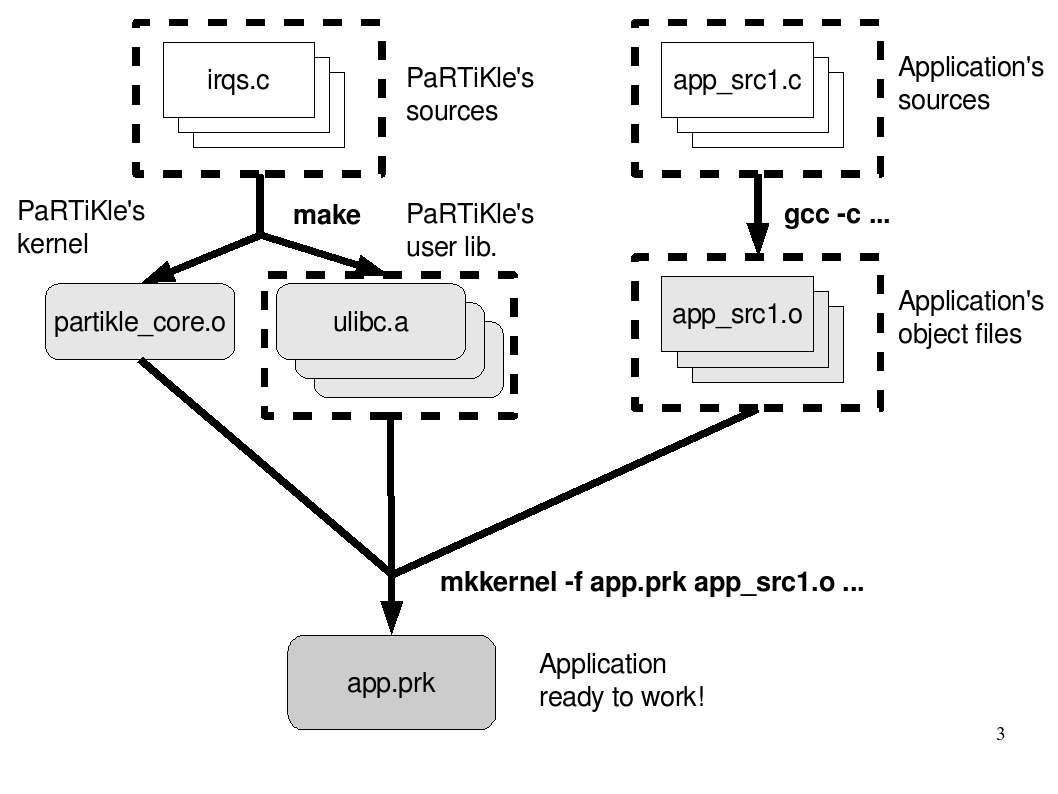
\includegraphics[width=0.5\textwidth]{img/partikle_building}
\caption{Configuration screen-shoots.}
\label{img:building}
\end{figure}


Invoking directly the compiler is not the most convenient way to build
an application. It is advisable to use \textit{make} (or other
dependency manager) to build complex. You can use the following
Makefile as a template:


\begin{lstlisting}[language=make,basicstyle=\small,framexrightmargin
    =-14mm,xleftmargin=14mm]
##################################################################
#                    Customisable section                        #
##################################################################

#### Name of the target file.
TARGET        := application.prtk

#### Path to the PaRTiKle root (it can be relative or absolute)
PaRTiKle_PATH := ../../../../partikle

#### All the ``C'' files of the current folder are part of the application.
#### SOURCES can be a explicit list of files.
SOURCES       := $(wildcard *.c)

#### Commen the followin line to compile quietly.
V             := 1

##################################################################
#                   Not customisable section                     #
##################################################################

OBJECTS       := $(addsuffix .o, $(basename $(SOURCES)))

all: $(TARGET)

$(TARGET): $(OBJECTS)
	$(LDKERNEL) -f $@  $<

%o: %c
	$(CC) $(CFLAGS) -c -o $@  $<

clean:
	rm -f *.prtk *.ktr *.o *~

include $(PaRTiKle_PATH)/config.mk
include $(PaRTiKle_PATH)/user/rules.mk
\end{lstlisting}

This \texttt{Makefile} can be found in the PaRTiKle distribution in
the folder: \texttt{user/examples/template}. You can move (copy) the
template folder to some place outside the PaRTiKle tree. In this case,
do not forget to update the \texttt{PaRTiKle\_PATH} variable of the
Makefile.

\section{Tracing PaRTiKle}

Tracing does ease the validation of the execution of any real-time
application. Currently, PaRTiKle supports tracing application when
running in a Linux execution environment\footnote{So far, tracing is
only supported in the Linux execution environment, however, it is
planned to support this feature in the other environments}. This
section presents a step by step guide to enable and to visualise the
resulting traces.
 
To support tracing, once enabled, PaRTiKle generates an extra file
named \textit{sched\_trace.ktr}. This file contains a sequence of
trace logs jointly with the time when they took place.

In order to analyse this data, PaRTiKle includes the
kiwi~\ref{kiwi} graphical tool.

\subsection{Configuration options}

Setting the option \verb+CONFIG_PORT_DEVTRACE+ in the configuration menu
enables the tracing support in PaRTiKle. Internally, selecting this
option means that the function \texttt{log\_event()} is called,
printing in a file named \textit{sched\_trace.ktr} each event as a
kiwi event.

\subsection{Using kiwi}\label{kiwi}

\href{http://rtportal.upv.es/apps/kiwi/}{Kiwi}
is a graphic application which displays tasks execution trace logs.
It has been entirely written in Tcl/TK, which makes it very portable.
Its main features are: impressive zoom, rich set of graphical elements,
output to eps files, events driven navigation and full customizable colors.
Kiwi is mainly focused on real-time systems,
but you can use it for represent any kind of concurrent application or system.

\begin{figure}[htbp]\centering
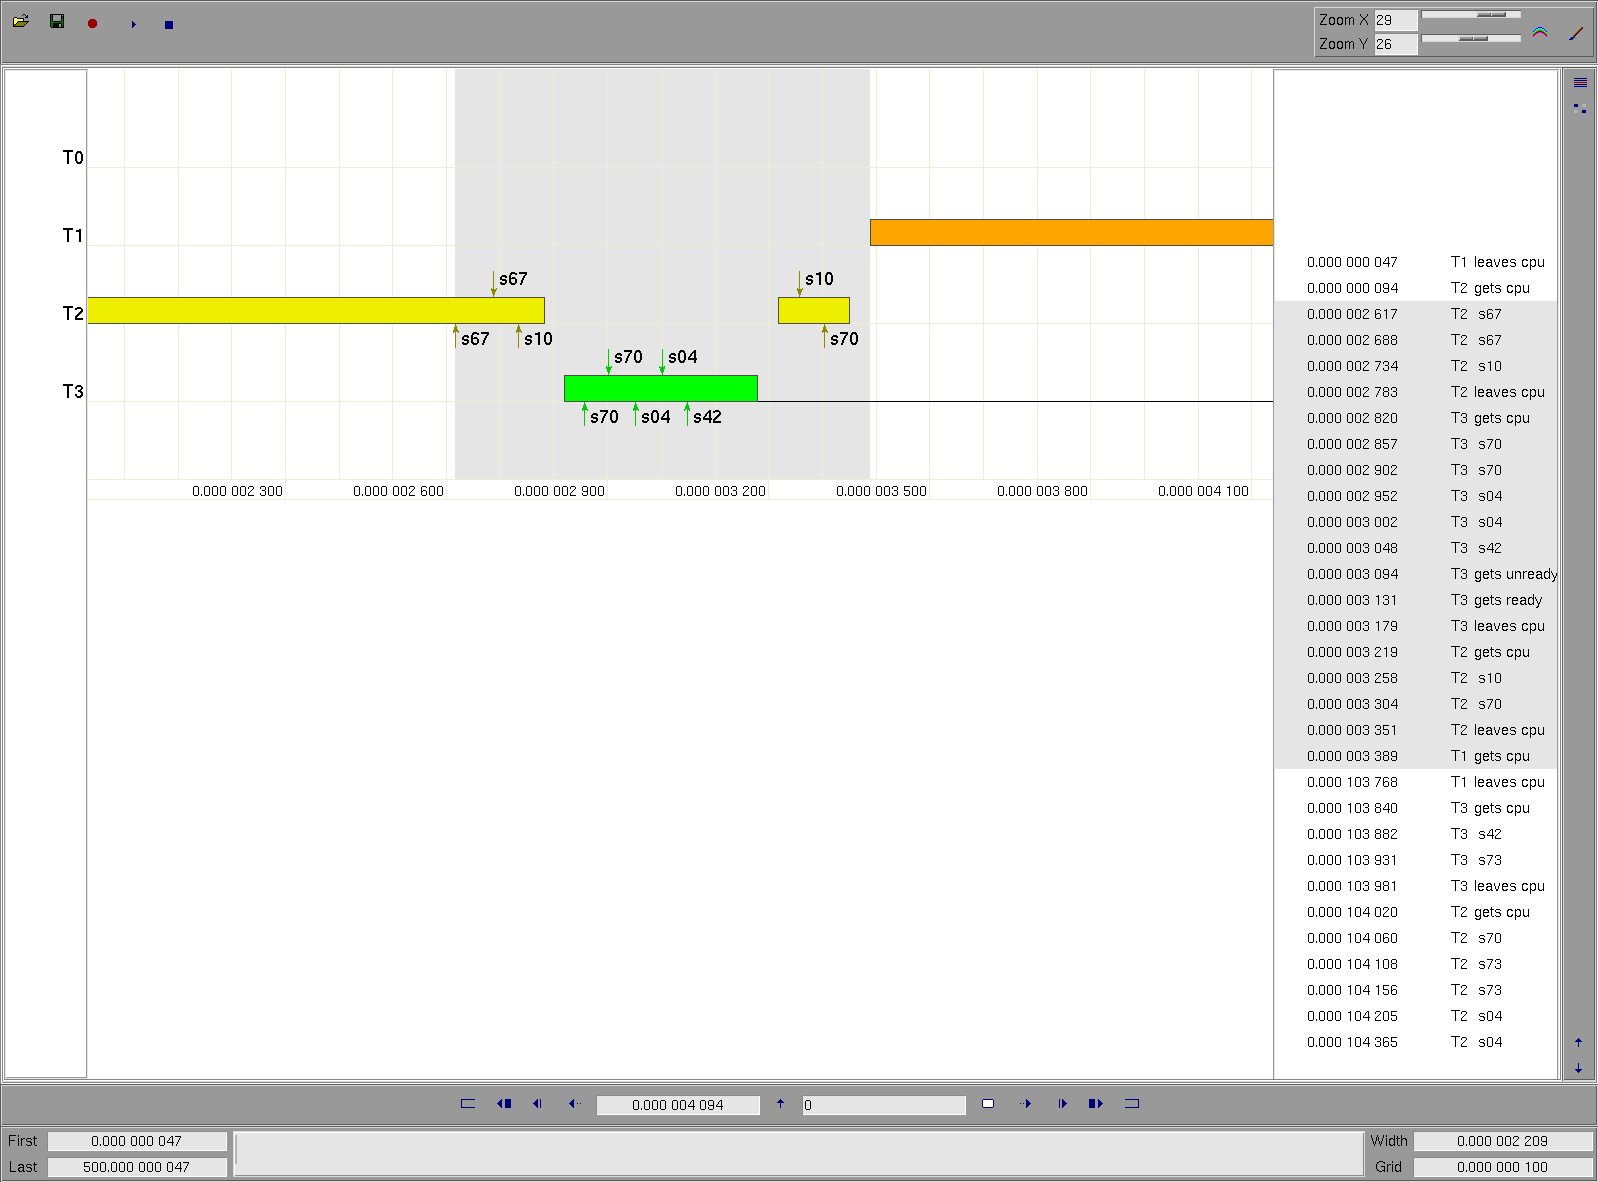
\includegraphics[width=0.49\textwidth]{img/kiwi}
\caption{kiwi showing context switches while accessing a shared resource}
\label{img:kiwi}
\end{figure}


To analyse a \textit{sched\_trace.ktr} file, kiwi can be run from command-line with:
\begin{verbatim}
    $ kiwi <sched_trace.ktr>
\end{verbatim}


\appendix

\chapter{Application example}\label{partikle:example}

The code below creates a single thread, waits for ten seconds, and
then cancels the thread. The thread prints every second its reference.
\begin{lstlisting}[basicstyle=\small,framexrightmargin
    =-14mm,xleftmargin=14mm,morekeywords={movl, testl, je, call}]

#include <stdio.h>
#include <stdlib.h>
#include <time.h>
#include <pthread.h>

void *thread_main(void *args) {
     struct timespec sleeping_time = {1, 0}, remaining;

     while (1) {
          printf ("I'm task1: %p\n",  pthread_self ());
          if (nanosleep (&sleeping_time, &remaining) == -1)
               printf ("remaining: seg %d nseg: %d\n", 
                       remaining.tv_sec, 
                       remaining.tv_nsec);
     }
     return (void *)0;
}

int main (int argc, char **argv) {
     pthread_t task1;
     struct timespec timeout = {10, 0};

     pthread_create (&task1, NULL, thread_main, NULL);
     nanosleep (&timeout, NULL);

     printf ("Request to finish\n");

     pthread_cancel (task1);
     pthread_join (task1, NULL);
     return 0;
}

\end{lstlisting}



\chapter{system calls}\label{parsyscall}
\begin{longtable}{|l|l|}\hline 
\multicolumn{1}{|c|}{Function} & \multicolumn{1}{c|}{Description} \\ \hline
\endhead
\texttt{pthread\_create} & create a new thread\\
\texttt{pthread\_exit} & terminate the calling thread\\
\texttt{pthread\_join} & wait for termination of another thread\\
\texttt{pthread\_detach} & put a running thread in the detached state\\
\texttt{pthread\_once} & once-only initialisation \\
\texttt{pthread\_self} & return identifier of current thread\\
\texttt{pthread\_equal} & compare two thread identifiers\\ \hline

\texttt{pthread\_setschedparam} & control thread scheduling parameters\\
\texttt{pthread\_getschedparam} & control thread scheduling parameters\\ \hline
\texttt{sched\_get\_priority\_max} & get maximum static priority range \\
\texttt{sched\_get\_priority\_min} & get minimum priority range\\
\texttt{pthread\_yield} & releases the processor\\ \hline


\texttt{pthread\_attr\_init} & initialize threads attributes object\\
\texttt{pthread\_attr\_destroy} & destroy threads attributes object\\
\texttt{pthread\_attr\_setstackaddr} & set stackaddr attribute \\
\texttt{pthread\_attr\_getstackaddr} & get  stackaddr attribute\\
\texttt{pthread\_attr\_setdetachstate} & set detachstate attribute  \\
\texttt{pthread\_attr\_getdetachstate} &  get  detachstate attribute \\
\texttt{pthread\_attr\_setinheritsched} & set/get scheduling policy and scheduling parameters \\
\texttt{pthread\_attr\_getinheritsched} & set/get scheduling policy and scheduling parameters \\
\texttt{pthread\_attr\_setschedpolicy} &set/get scheduling policy and scheduling parameters \\
\texttt{pthread\_attr\_getschedpolicy} & set/get scheduling policy and scheduling parameters\\
\texttt{pthread\_attr\_setschedparam} & set/get scheduling policy and scheduling parameters\\
\texttt{pthread\_attr\_getschedparam} & set/get scheduling policy and scheduling parameters\\ \hline

\texttt{pthread\_setcancelstate} & set cancelability state  \\
\texttt{pthread\_cancel} & cancel execution of a thread\\
\texttt{pthread\_cleanup\_push} & establish cancelation handlers\\
\texttt{pthread\_cleanup\_pop} & remove cancelation handlers\\ \hline


\texttt{pthread\_mutex\_init} & initialize a mutex \\
\texttt{pthread\_mutex\_destroy} & destroy and initialize a mutex \\
\texttt{pthread\_mutex\_lock} & lock a mutex \\
\texttt{pthread\_mutex\_trylock} & try to lock a mutex  \\
\texttt{pthread\_mutex\_timedlock} &  lock a mutex with timeout\\
\texttt{pthread\_mutex\_unlock} & unlock a mutex\\ \hline

\texttt{pthread\_mutex\_setprioceiling} &  set the priority ceiling of a mutex \\ 
\texttt{pthread\_mutex\_getprioceiling} & get the priority ceiling of a mutex\\ \hline
  


\texttt{pthread\_mutexattr\_init} &  initialize mutex attributes object\\
\texttt{pthread\_mutexattr\_destroy} & destroy and initialize mutex attributes object\\
\texttt{pthread\_mutexattr\_setprotocol} & set protocol attribute of mutex attributes object \\
\texttt{pthread\_mutexattr\_getprotocol} & get  protocol attribute of mutex attributes object \\
\texttt{pthread\_mutexattr\_setprioceiling} & set prioceiling attribute of mutex attributes object \\
\texttt{pthread\_mutexattr\_getprioceiling} & get prioceiling attribute of mutex attributes object\\
\texttt{pthread\_mutexattr\_settype} & set a mutex type attribute\\
\texttt{pthread\_mutexattr\_gettype} & get a mutex type attribute\\ \hline

\texttt{pthread\_cond\_init} &  initialize condition variables\\
\texttt{pthread\_cond\_destroy} & destroy and initialize condition variables\\
\texttt{pthread\_cond\_signal} & signal a condition\\
\texttt{pthread\_cond\_broadcast} & broadcast or signal a condition\\
\texttt{pthread\_cond\_wait} &  wait on a condition\\
\texttt{pthread\_cond\_timedwait} & wait on a condition with timeout\\ \hline

\texttt{pthread\_condattr\_init} & initialize condition variable attributes object\\
\texttt{pthread\_condattr\_destroy} & destroy and initialize condition variable attributes object\\ \hline

\texttt{pthread\_key\_create} & thread-specific data key creation\\
\texttt{pthread\_key\_delete} & thread-specific data key deletion\\
\texttt{pthread\_setspecific} & thread-specific data management\\
\texttt{pthread\_getspecific} & thread-specific data management\\ \hline

\texttt{sigaction} & examine and change signal action\\
\texttt{sigqueue} & queue a signal to a process \\
\texttt{pthread\_kill} &  send a signal to a thread\\
\texttt{pthread\_sigmask} &  examine and change blocked signals \\
\texttt{sigwait} & wait for queued signals\\
\texttt{sigsuspend} & wait for a signal\\
\texttt{sigpending} &  examine pending signals\\ \hline

\texttt{sigemptyset} & initialize and empty a signal set \\
\texttt{sigfillset} &  initialize and fill a signal set \\
\texttt{sigaddset} & add a signal to a signal set\\
\texttt{sigdelset} & delete a signal from a signal set\\
\texttt{sigismember} & test for a signal in a signal set\\
\texttt{sigismember} & test for a signal in a signal set\\ \hline

\texttt{mktime} & convert broken-down time into time since the Epoch\\
\texttt{localtime\_r} &convert a time value to a broken-down local time \\
\texttt{localtime} & convert a time value to a broken-down local time\\
\texttt{nanosleep} & pause execution for a specified time
 \\
\texttt{usleep} & suspend execution for microsecond intervals\\
\texttt{clock\_settime} & set the time of a given block \\
\texttt{clock\_gettime} & get the time of a given block\\
\texttt{clock\_getres} & get the resolution of any clock \\
\texttt{gettimeofday} & get time\\ \hline

\texttt{open} & open a file \\
\texttt{close} & close a file \\
\texttt{read} & read bytes from a file \\
\texttt{write} & write bytes to a file \\ \hline

\texttt{install\_irq\_handler} & install a handler to manage an interrupt \\
\texttt{install\_trap\_handler} & install a handler to manage a trap \\
\texttt{hw\_disable\_irq} & disable an interrupt  \\
\texttt{hw\_enable\_irq} & enable an interrupt \\
\texttt{hw\_ack\_irq} & acknowledged an interrupt \\
\texttt{hw\_end\_irq} & end the management of an interrupt \\
\texttt{hw\_cli} & disable all interrupts \\
\texttt{hw\_sti} & enable all interrupts \\
\texttt{hw\_restore\_flags} & restore system's flags \\
\texttt{hw\_save\_flags} & save system's flags \\
\texttt{hw\_save\_flags\_and\_cli} & save system's flags and disable interrupt \\ \hline

\texttt{dirname} & strip non-directory suffix from file name\\
\texttt{basename} & strip directory and suffix from filenames\\ \hline


\texttt{getpid} & get process identification \\
\texttt{getppid} &get parent process identification \\ \hline

\texttt{malloc} & allocate dynamic memory\\
\texttt{free} & release dynamic memory\\
\texttt{realloc} & change the size of a block\\
\texttt{calloc} & allocate dynamic memory\\ \hline

\texttt{mmap} & allocate a chunk of memory (only flag \texttt{MAP\_ANONYMOUS})\\
\texttt{munmap} &  deallocate a previously allocated chunk of memory \\ \hline

\texttt{memset} & fill memory with a constant byte\\
\texttt{memcpy} & copy memory area\\
\texttt{memmove} & copy memory area\\
\texttt{strcpy} & copy a string\\
\texttt{strncpy} & copy a string. bounded \\
\texttt{strcat} & concatenate two strings\\
\texttt{strcmp} & compare two strings\\
\texttt{strlen} & calculate the length of a string\\
\texttt{strchr} & locate character in string\\
\texttt{strrchr} & locate character in string. reverse search \\
\texttt{strstr} & locate a substring\\ \hline


\texttt{printf} & format and print data\\
\texttt{putchar} &output of characters \\
\texttt{sscanf} & input format conversion\\
\texttt{scanf} & input format conversion\\
\texttt{fgetc} & input of characters\\
\texttt{ungetc} & push a character back\\
\texttt{fputs} & output string\\
\texttt{puts} & output string\\
\texttt{sprintf} & format and print data\\ \hline
\end{longtable}

\end{document}
